\chapter{Uvod} \label{uvod}

Skozi celotno zgodovino so si ljudje želeli olajšati fizična dela na različne načine. Ponavljajoča dela je olajšala uporaba pogonov. Električni pogoni so delovne procese optimizirali. Za točnejše delovanje so se razvili različni načini krmiljenja. Z novimi načini krmiljenja, so se pojavile tudi potrebe po merjenju novih količin. V zadnjih desetletjih, je pri krmiljenuju, potrebna informacija o trenutnem položaju pogona.

Trenutni položaj merijo dajalniki pomika ali zasuka\cite{uporabaSenzorjev}. Pri rotacijskih dajalnikih ločimo dajalnike, ki merijo zasuk na koncu osi (angl.: on axis) in dajalnike, ki merijo zasuk na osi (angl.: through hole). Možna delitev rotacijskih dajalnikov je tudi na eno-obratne (angl.: single-turn) in več-obratne (angl.: multi-turn). Eno-obratni rotacijski dajalniki podajo položaj znotraj enega obrata, medtem ko več-obratni štejejo tudi število polnih obratov. Dajalnike položaja delimo tudi glede na uporabljeni princip zaznavanja fizikalne
spremembe, torej glede na uporabljeno tehnologijo. Poznamo magnetne, optične,
induktivne in druge\cite{killer}.

Pri magnetnem principu senzor dajalnika zaznava spremembo jakosti in smeri
magnetnega polja. 
Magnetno polje se ustvari z aktuatorjem radialno polariziranega magneta. Meri se s Hallovimi sondami ali AMR senzorji. Iz zajetega polja sledi izračun dejanskega položaja. Dajalnik položaja, ki pretvarja merjeno magnetno polje v informacijo o položaju imenujemo enkoder\cite{enkoder}.

Kot vsak merilni element, ima tudi magnetni enkoder napako. Napaka se lahko pojavi ob narobe merjenem magnetnem polju\cite{RLS3}. Napako lahko povzroči tudi napačno pomerjeno polje. To se zgodi ob nepravilni montaži enkoderja ali magnetnega aktuatorja na pogon. S poznavanjem vplivov nepravilne montaže na napako pomerjenega položaja, se napako lahko predvidi in odpravi.

Cilj naloge je analizirtai kako različne napake pri montaži, vplivajo na napako v signalih kota.
Želi se predstaviti čimbolj preprost model, ki bo dovolj točno opisal dogajanje ob prisotnosti napake in to prekontrolirati.

%Senzor RM44 mora biti za pravilno delovnanje in točnost izhodnega podatka pravilno montiran.% V podatkovnih listih je podana toleranca $\pm100\mathrm{\mu m}$. 

%Magistrsko delo predstavlja vpliv nepravilno montiranega senzorja ali nepravilno montiranega magneta na napako.





%V tej magistrski nalogi je predstavljen vpliv napačno merjenega magnetnega polja. Predstavljen je simulacijski model enkoderja, ter odvistnost napake na nepravilno montažo. Simulacije so primerjane z meritvami na enkoderju RM44\cite{RM44}.


\chapter{Senzor RM44}

Senzor RM44 je 13 bitni enkoder, primeren za merjenje zasuka rotirajočega pogona\cite{RM44}.
Enkoder se nahaja v robustem ohišju, zato je primeren za delovanje v težkem industrijskem okolju. % , pritrjenega na konec rotirajoče osi pogonskega sklopa.
Oblika izhodnega podatka o zasuku, je prilagodljiva na sistem aplikacije v kateri bo uporabljen\cite{Ambrozic}. Izhod senzorja je lahko analogni v obliki sinusnega in cosinusnega signala ali linearno spreminjajče se napetosti med potencialoma GND in VDD v odvisnosti od kota zasuka.
Izhod je lahko tudi v oliki inkrementalnih signalov A in B s katerih se lahko določi smer in relativni zasuk vrtenja ter signal Ri kateri določa referenčno točko. Izhod je možen tudi preko SSI vodila. Senzor ima možnost nastavitev resolucije od 5 do 13 bitov \cite{AM8192}\cite{RM44}. Senzor na katerem so bile opravljene meritve je imel na voljo analogna signala sinus in kosinus. Točno ime senzorja je RM44AC0001S20F2E10, v delu bo poimenovan okrajšano RM44.
\begin{figure}[h]
	\centering
	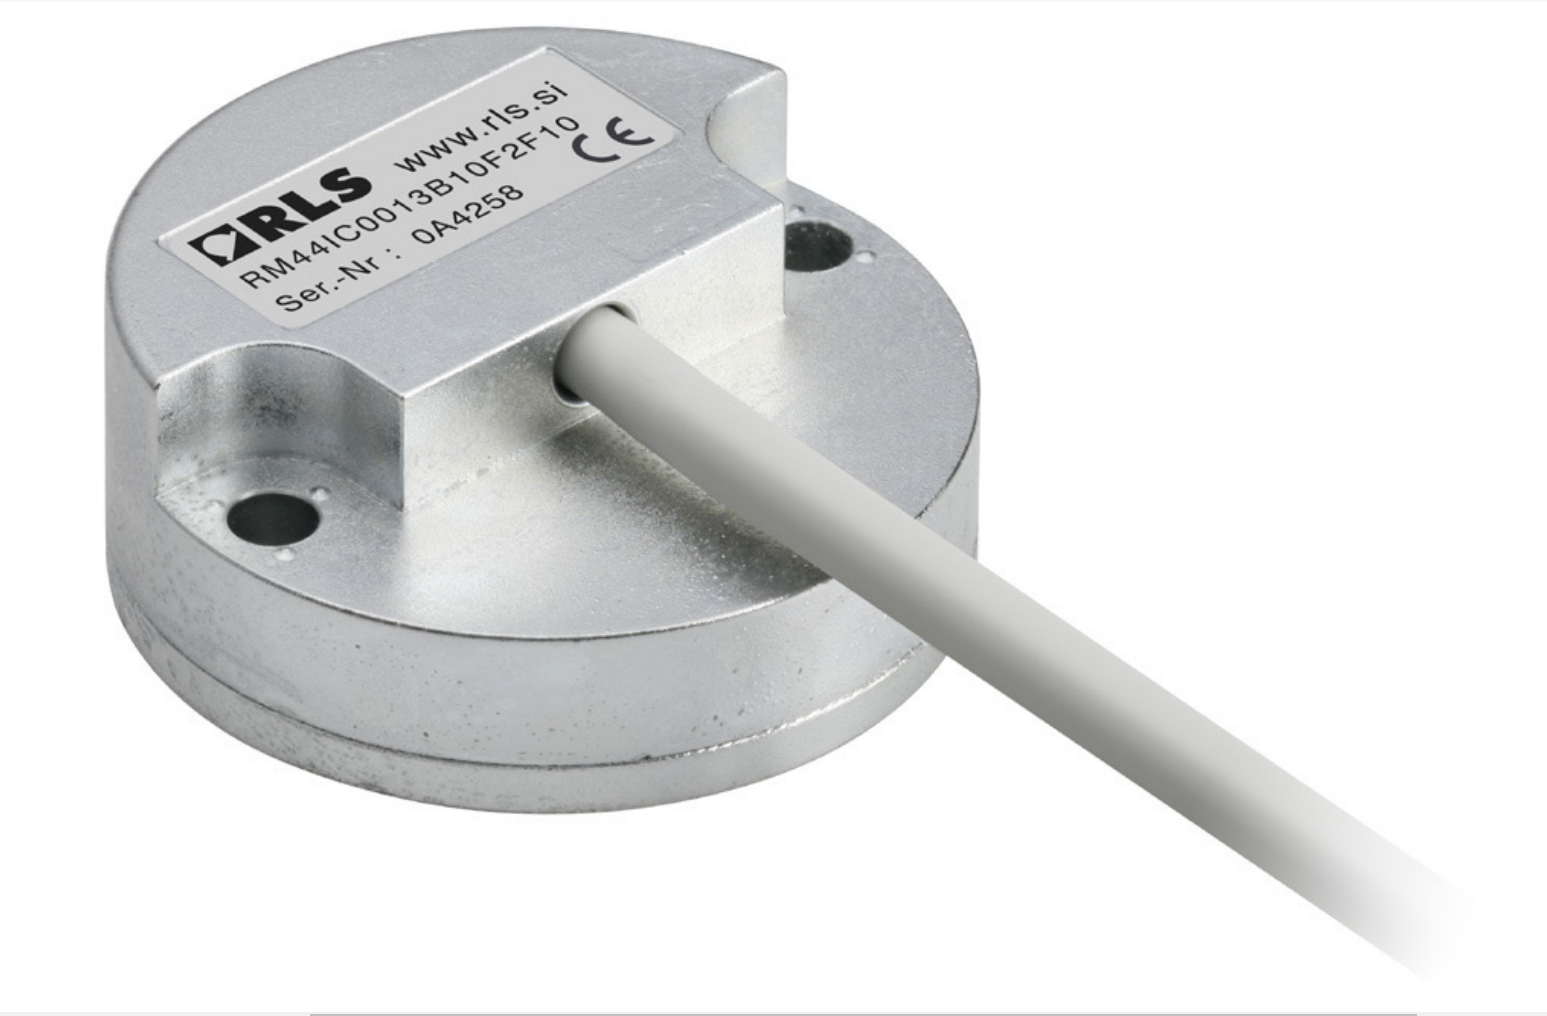
\includegraphics[width=0.6\columnwidth]{./Slike/senzorRM44.jpg}
	\caption{Senzor RM44}
	\label{RM44}
\end{figure}

Ključni element senzorja je čip AM256. Za odčitavnaje zasuka, se mora nahajati nad radialno polariziranim cilindričnim magnetom, ki je pritrjen na os vrtenja(slika \ref{stranski_ris}).
S strani proizvajalca senzorja je priporočen radialno polariziran magnet s premerom 4 mm in višino 4 mm (slika \ref{magnet4mm}).
\begin{figure}[h]
	\centering
	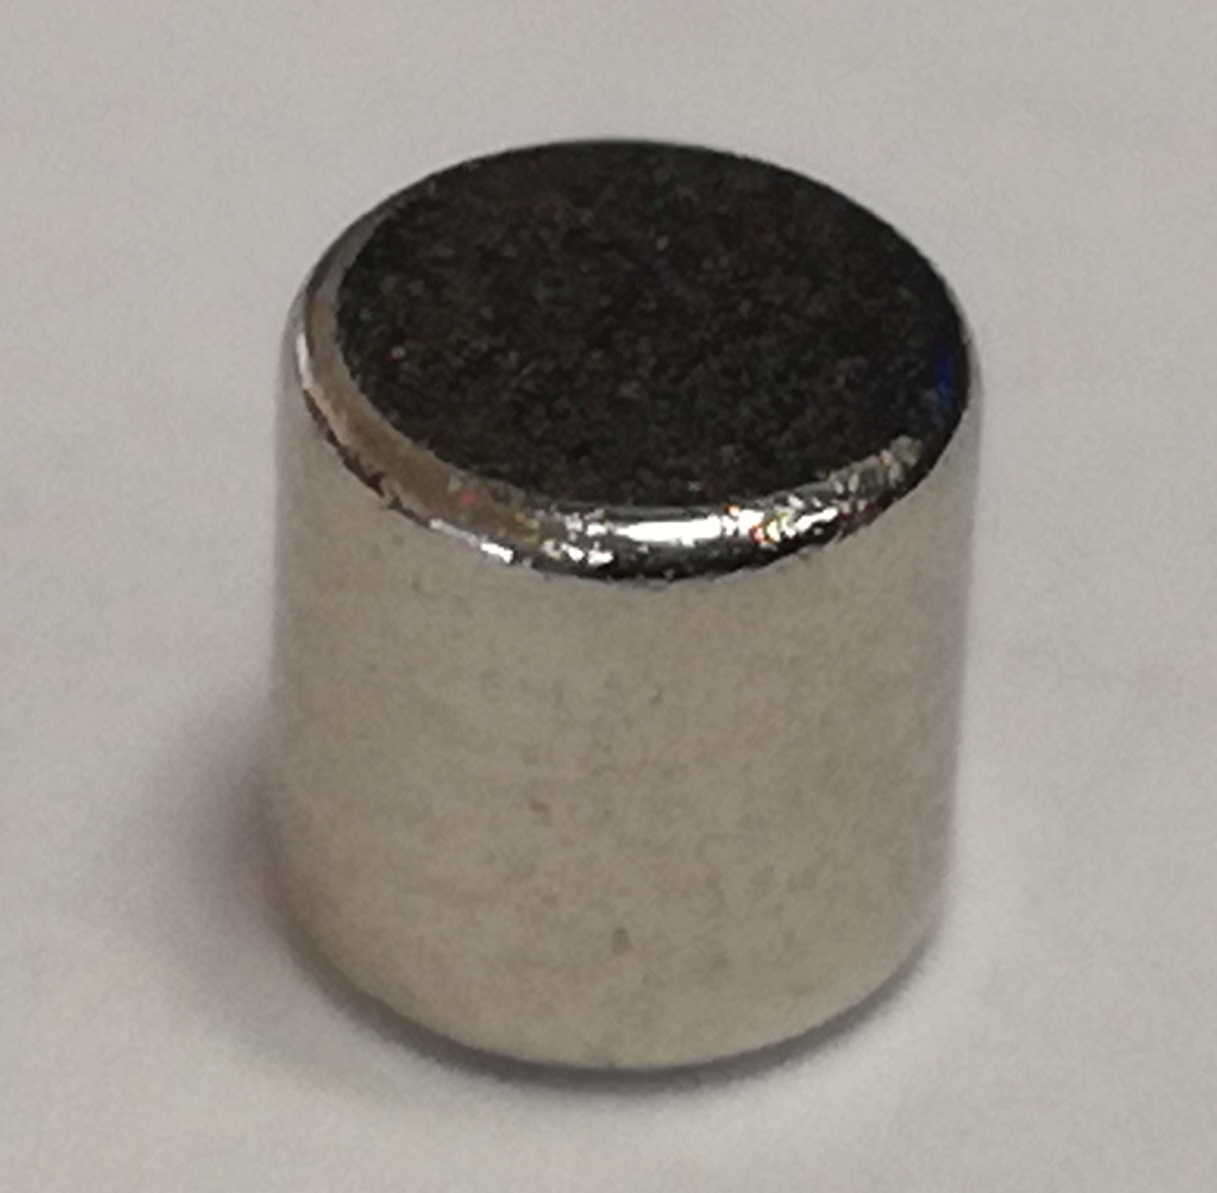
\includegraphics[width=0.35\columnwidth]{./Slike/magnet4mm.png}
	\caption{Primer magneta predlagan s strani proizvajalca RLS}
	\label{magnet4mm}
\end{figure}

Na siliciju čipa so razporejene Hallove sonde za meritev Z-komponento gostote magnetnega pretoka. Za merjenje Z-komponento gostote magnetnega pretoka je lahko čip obrnjen kot na sliki \ref{stranski_ris}, ali obrnjen na glavo. Med silicijevo rezino in magnetom se pri taki montaži nahaja še tiskanina. Tiskanina nima magnetnih lastnosti in ne vpliva na meritve Hallovih sond. Pri montiranju je potrebno ohraniti predpisano razdaljo med magnetom in silicijevo rezino ($1,8 \mathrm{mm}$).

\begin{figure}[h]
	\centering
	\includegraphics[width=0.5\columnwidth]{./Slike/stranski_ris.png}
	\caption{Nahajanje radialno polariziranega magneta nad čipom AM256 \cite{AM8192}}
	\label{stranski_ris}
\end{figure}

Na sliki \ref{polje_brez_ravnine}  je prikazana oblika Z komponente vektorja gostote magnetnega pretoka povzročene z radialno polariziranim cilindričnim magnetom.
\begin{figure}[h]
	\centering
	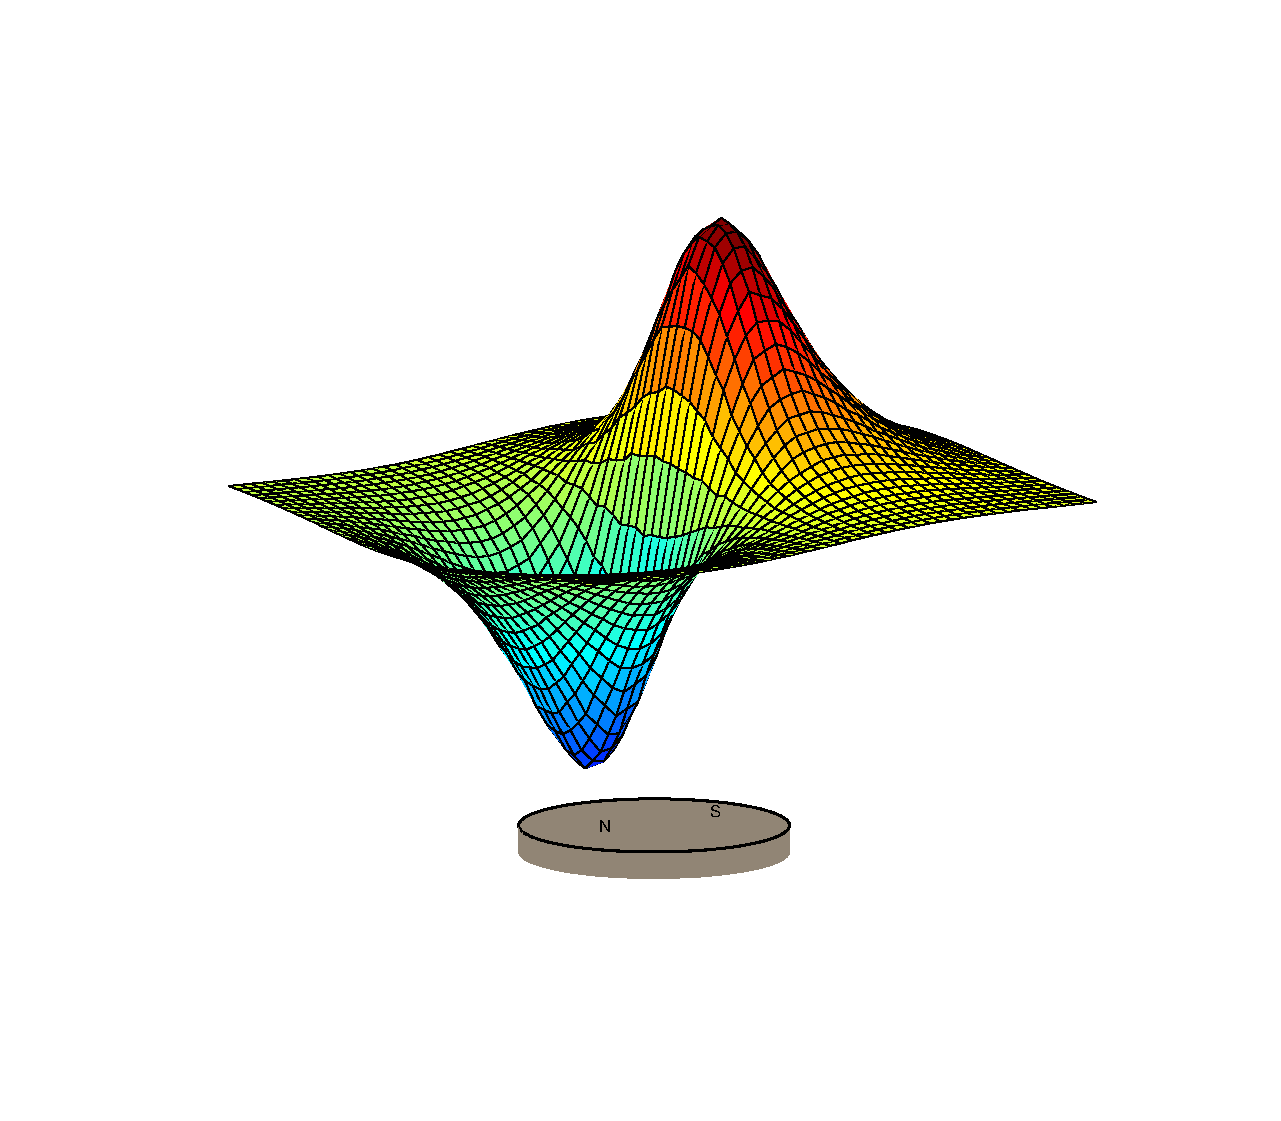
\includegraphics[width=\columnwidth]{./Slike/polje_brez_ravnine.eps}
	\caption{Oblika Z komponente gostote magnetnega pretoka nad magnetom}
	\label{polje_brez_ravnine}
\end{figure}
Slika \ref{polje_brez_ravnine} prikazuje rezultat Z-komponente gostote magnetnega pretoka simuliranega magneta, ki ga priporoča proizvajalec senzorja.

S pravilno postavitvijo Hallovih sond in obliki Z-komponente gostote magnetnega pretoka povzročene z magnetom, se ob prostorskem zajemu zajame 2 signala kosinusne oblike, ki sta za 90$^\circ$ prostorsko zamaknjena drug na drugega (slika \ref{BxBy}). Prvi zajet signal,  fazno prehiteva za 90$^\circ$ drugi signal in je v delu poimenovan $B_{cos}$, drugi signal, je poimenovan $B_{sin}$.
\begin{figure}[h]
	\centering
	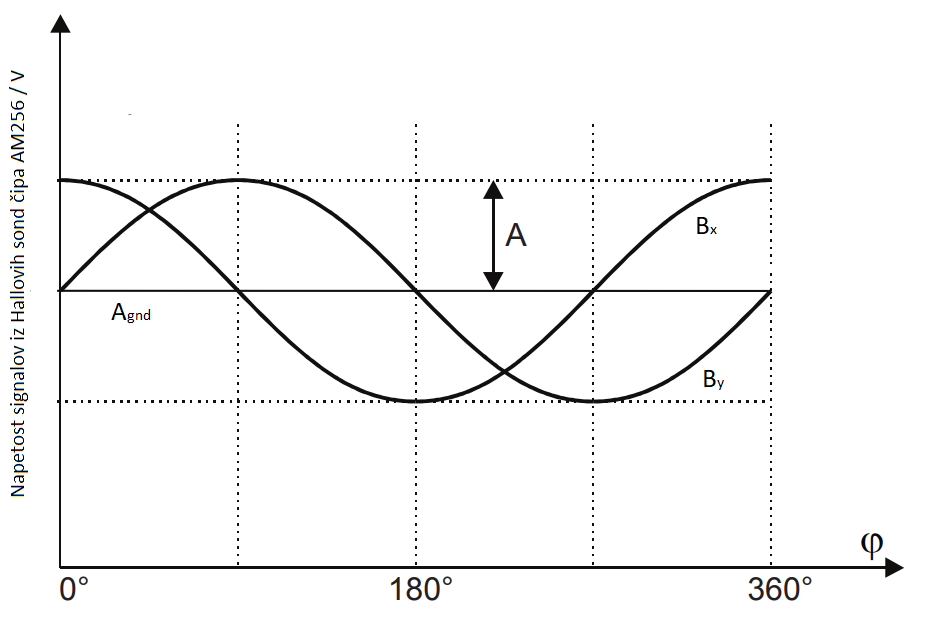
\includegraphics[width=0.7\columnwidth]{./Slike/BxBy.png}
	\caption{Analogna signala zajeta s Hallovimi sondami \cite{AM8192}}
	\label{BxBy}
\end{figure}

Iz signalov, zajetih s Hallovih sond, se izračuna kot. Metod, za numeričen izračun kota iz podatkov kot sta signala $B_{cos}$ in $B_{sin}$ je več (CORDIC, SAR, sledilna metoda, itd \cite{ICHaus_interpolate}). Osnovni princip metode je izračun funkcije atan2($B_{sin}$, $B_{cos}$) \cite{atan2Matlab}.

Osnovno delovanje senzorja se lahko ponazori, z dvema Hallovima sondama.  Sondi sta postavljeni na krožnico s središčem v osi vrtenja magneta in radijem $r_0$.

Sondi sta prostorsko zamaknjeni za 90$^\circ$ (slika \ref{opis_modela}).  S sondama se zajame signala $B_{cos}$ in $B_{sin}$. Signala sta vhodna parametra v funkcijo atan2(), ki izračuna kot zasuka (slika \ref{opis_modela}). Za oceno napake, se lahko Z komponento gostote magnetnega pretoka v okolici središča magneta, aproksimira z ravnino (slika \ref{polje_z_ravnino}).
\begin{figure}[h]
	\centering
	\includegraphics[width=0.9\columnwidth]{./Slike/polje_z_ravnino.eps}
	\caption{Oblika Z komponente gostote magnetnega pretoka nad magnetom in aproksimirano ravnino v središču magneta}
	\label{polje_z_ravnino}
\end{figure}
\begin{equation}
\label{equ:poljeB1}
B_z(x,y)=k\cdot x.
\end{equation} 



Aproksimacija zadostuje za oceno napake. S poznavanjem lokacije sonde glede na magnet, se lahko izračuna merjena komponenta magnetnega polja. Aprokisimirano polje je linearno odvisno od x komponente (\ref{equ:poljeB1}). Za lažje razumevanje bo $k$ enak $1\frac{\mathrm{mT}}{\mathrm{mm}}$.

\begin{figure}[h]
	\centering
	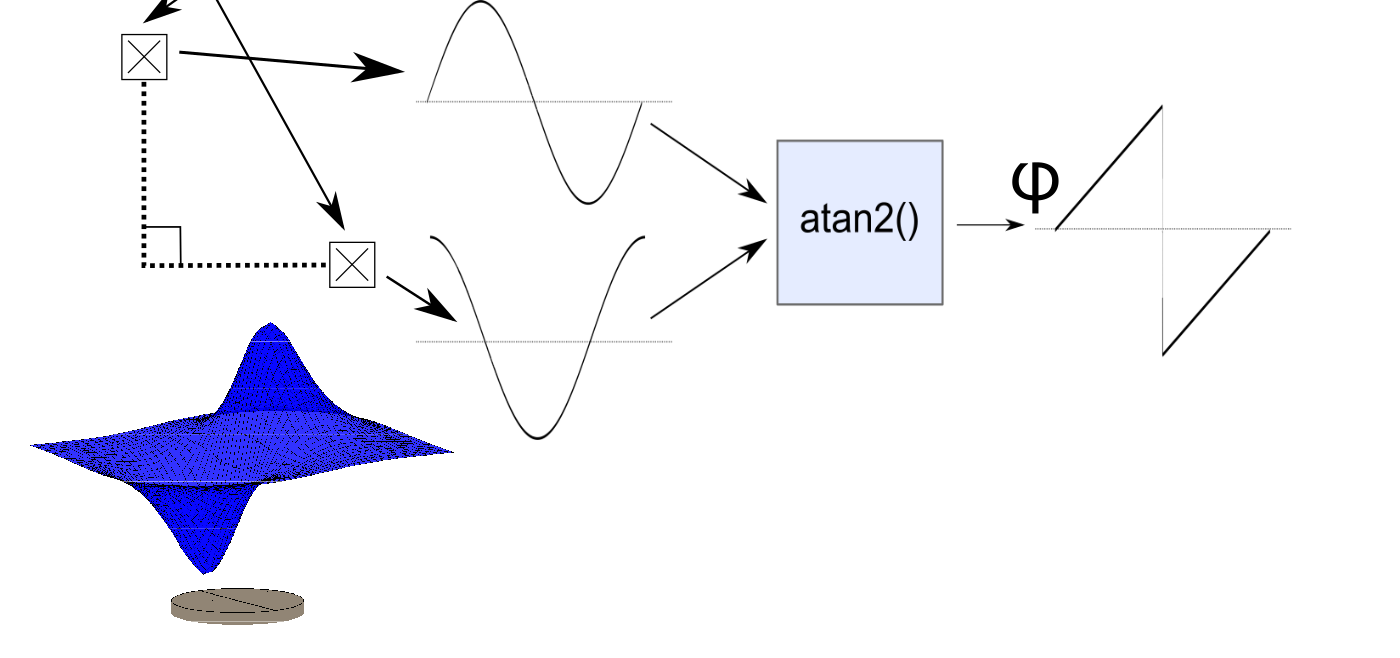
\includegraphics[width=0.9\columnwidth]{./Slike/opis_modela.png}
	\caption{Osnovni model, za izračun kot zasuka}
	\label{opis_modela}
\end{figure}
%
%Senzorji se delijo resolverje in enkoderje. Resolver ima unikatno oblikovan rotorski aktuator, kjer se med vretenjem zaradi posebne oblike, zračna reža spreminja sinusno. To ima za posledico istovrstno spreminjanje upornosti magnetnih poti fluksa med primarnimi in sekundarnimi glavami navitij ter nato induciranih napetosti \cite{Ursic}.
%
%
%delijo na absolutne ali inkrementalne merilnike. Inkrementalni nam sporočijo relativo spremembo zasuka, ob prehodu referenčne točke se lahko senzor šele inicializira in od takrat dalje je možen izračun dejsanskega zasuka. Primer takega senzorja je optični senzor zasuka.
%
%Absolutni dajalniki zasuka lahko neglede na dan zasuk razbere dejansko vrednost zasuka rotorja. Primera sta 
%
%Enkoder oz. rotacijski enkoder je naprava 